\documentclass[11pt]{article}

\usepackage{graphicx}
\usepackage{amsmath}
\usepackage{amsfonts}
\usepackage{amssymb}
\usepackage{amsxtra}
\usepackage{bm}
\usepackage{lineno}
\usepackage{url}
\usepackage{setspace}
\usepackage[title]{appendix}
\usepackage[a4paper, margin=1in]{geometry}
\usepackage[dvipsnames]{xcolor}
\usepackage[protrusion=true, expansion=true]{microtype}
\usepackage[authoryear]{natbib}
\usepackage[bf, font={small}]{caption}
\usepackage[T1]{fontenc}
\usepackage[utf8]{inputenc}
\usepackage{lmodern}

\newcommand{\ud}{\mathrm{d}}
\newcommand{\e}{\mathrm{e}}
\newcommand{\SI}{Supplementary}
\newcommand{\ol}[1]{\overline{#1}}
\newcommand{\rem}[1]{\textcolor{red}{\textrm{#1}}}
\newcommand{\citeapos}[1]{\citeauthor{#1}'s (\citeyear{#1})}
\let\originalleft\left
\let\originalright\right
\renewcommand{\left}{\mathopen{}\mathclose\bgroup\originalleft}
\renewcommand{\right}{\aftergroup\egroup\originalright}

\clubpenalty = 10000
\widowpenalty = 10000
\bibpunct{(}{)}{,}{a}{}{,}
\graphicspath{{../figures}}
\allowdisplaybreaks


\begin{document}

\title{When do trait-based higher-order interactions and individual variation promote robust species coexistence?}
\author{Gaurav Baruah$^{ \ddag, \ast,1}$, Gy\"orgy Barab\'as$^{\ddag, 2,3}$, Robert John$^4$}
\date{}

\maketitle

\doublespacing

\noindent $^1$Faculty of Biology, Theoretical Biology, University of Bielefeld, 33501 Bielefeld, Germany

\noindent $^2$Division of Biology, Link\"oping University, Link\"oping, Sweden

\noindent $^3$Institute of Evolution, Centre for Ecological Research, Budapest, Hungary

\noindent $^4$Department of Biological Sciences, Center for Climate and Environmental Studies, IISER Kolkata, India

\noindent $^\ast$Corresponding author (email: \texttt{gbaruahecoevo@gmail.com}, )

\noindent $^{\ddag}$ shared first authorship.

\bigskip



\bigskip


\noindent \textbf{Keywords:} higher-order interactions, intraspecific variation, eco-evolutionary dynamics, species coexistence, trait clustering, stability

\newpage{}
\linenumbers


\begin{abstract}
\noindent Models on the effects of individual variation often focus on pairwise interactions, but communities could harbor both pairwise and higher-order interactions (HOIs). Theoretical studies that do consider HOIs tend to assign them at random, even though they could be mediated and structured by traits. Here we consider two different classes of models of both pairwise and higher-order trait-mediated interactions: competition alleviated by increasing trait distance, and hierarchical competition where species higher in the hierarchy exert more competition on those lower and vice versa. Combining these models with evolutionary dynamics based on quantitative genetics, we compare their impact on species diversity, community pattern, and robustness of coexistence. Regardless of individual variation, trait-mediated HOIs generally do not promote and often hinder species coexistence, but there are some notable exceptions to this. We present an analytical argument to make sense of these results, and argue that while the effects of trait-based HOIs on diversity may appear confusing on the surface, we can understand what outcome to expect in any given scenario by looking at the shape of the effective interaction kernel that arises from the joint action of pairwise and HOI terms. Apart from this, we also find that (i) communities structured by trait hierarchies are particularly vulnerable to external perturbations, irrespective of the presence of HOIs; (ii) trait-based HOIs with distance-dependent competition result in communities that are the most robust to external perturbations compared to other communities, with individual variation having minimal impact on this robustness; and (iii) both individual variation and HOIs consistently lead to a more even distribution of species traits than would occur by chance. These findings suggest that one-dimensional trait-mediated HOIs foster coexistence only under special conditions, raising the question of whether HOIs must involve multiple traits to positively affect coexistence in competitive communities.
\end{abstract}


\newpage{}


\section{Introduction} \label{sec:intro}

Explanations for multispecies coexistence in ecological communities have largely been sought at the species level by emphasizing mean differences among species driven by competitive interactions or life-history trade-offs \citep{gravel_species_2011,violle_towards_2009,clark_high-dimensional_2010,kraft_plant_2015,valladares_species_2015}. The idea being that differences among species along multiple ecological dimensions would minimize niche overlap and permit long-term species coexistence \citep{barabas_effect_2016}. However, species often compete for only a small number of limiting resources 
\citep{hutchinson_paradox_1961,laird_competitive_2006, li_effects_2016-1,shoresh_evolution_2008, letten_mechanistic_2019}  and numerous species may coexist despite little differences in demographic or resource-based niches \citep{condit_importance_2006}, which poses a challenge for classical coexistence models. Such classical competition models of coexistence consider interactions between every possible pairing of species and require precise parameter
trade-offs to stabilize communities or to limit the strength of competition among coexisting species in accordance with the competitive exclusion principle 
 \citep{barabas_continuous_2012}. Theoretical studies with competition models further show that any stability achieved through strong self-regulation or strong intraspecific pairwise competitive interactions \citep{barabas_self-regulation_2017} can be disrupted by strong interspecific interactions among species. 

Competitive interactions among species are not always constrained to species pairs and can involve higher-order combinations \citep{wilson_complex_1992,laird_competitive_2006,grilli_higher-order_2017, mayfield_higher-order_2017}, where interactions between a species pair is modulated by one or more species. In an ecological system where pairwise interactions structure communities, higher-order interactions (HOIs) may modify these pairwise interactions and restructure communities \citep{levine_beyond_2017, singh_higher_2020}. For example, a superior competitor for a limiting resource will inhibit an inferior competitor for the same resource, but a third species may modulate the strength of this inhibition without affecting either of the two competitors directly \citep{bairey_high-order_2016}. Such attenuation of the pairwise inhibitory effect can be density-mediated or trait-mediated and can lead to qualitatively different community dynamics compared to the case with purely pairwise interactions \citep{grilli_higher-order_2017}. HOIs that have been studied thus far are mostly parameterized by assigning interaction coefficients that are sampled from random normal distributions \citep{bairey_high-order_2016, letten_mechanistic_2019}. With such random HOI structures, species coexistence is promoted provided the coefficients fulfill certain conditions \citep{singh_higher_2020}. Random HOIs could be termed ``high-dimensional'', because when a diversity of different independent species traits determine interaction coefficients, their values can often be modeled as being effectively random and independent of one another. By contrast, low-dimensional HOIs could come into effect when interactions are structured by just a handful of species traits. Indeed, in large communities, species interactions are dictated by traits species possess \citep{guimaraes_evolution_2011, maruyama_morphological_2014, mcpeek_evolutionary_2017} which consequently  could structure communities and impact stability \citep{barabas_effect_2016,baruah_impact_2022}. While the importance of such HOIs has been recognized \citep{levine_beyond_2017}, the nuances of such structured HOIs and competitive pairwise interactions in communities have proven difficult to study theoretically or empirically. 

The emphasis on pairwise species interactions in studies of coexistence is potentially limiting not just because pairwise interactions disregard HOIs, but also because of its focus on species and treating them as homogeneous units. Indeed, within-species trait variation is often ignored from species coexistence mechanisms \citep{siefert_incorporating_2012, hart_how_2016}.  It is now clear that intraspecific variation can have both ecological and evolutionary effects on competitive interactions, which ultimately determine patterns of species coexistence \citep{yamamichi_integrating_2022, pastore_evolution_2021}. For example, intraspecific trait variation can undermine species coexistence by increasing or decreasing competitive ability, niche overlap, and even-spacing among species \citep{barabas_effect_2016}, or by altering competitive outcomes through non-linear averaging of performances (Hart et al. 2016). There is equally compelling evidence that intraspecific variation promotes species coexistence whenever species have similar mean traits but different intraspecific trait variances \citep{bolnick_why_2011, barabas_effect_2016}. Experimental work has shown that although intraspecific variation allows a community to be resilient against invaders, it creates an opportunity for competitive exclusion among strong competitors \citep{hausch_effects_2018}. Empirical studies in the field have found, for instance, that leaf economic traits such as specific leaf area, leaf N and P consistently display high intraspecific variation \citep{meziane_interacting_1999}, and influence community assembly and ecosystem functioning \citep{reich_world-wide_2014}. Given that high levels of intraspecific trait variation within communities appear to be more a rule than an exception, the implications of intraspecific variation to community structure merits detailed investigation.

Clearly, both higher-order species interactions and intraspecific variation can have a significant influence on community structure, but these two properties have always been investigated separately in studies on species coexistence. The effects of intraspecific trait variation and eco-evolutionary dynamics on structuring large communities where both pairwise and HOIs dominate a community are therefore unexplored. Theoretical analyses indicate that purely pairwise interactions in a community lead to more even trait spacing than expected by chance. However, a community dominated by both pairwise and HOIs could lead to greater trait clustering along a trait axis. The apparent mechanism could be that with intraspecific variation present, HOIs can alleviate and stabilize the negative pairwise interactions that would otherwise lead to distinct spacing. One of our main goals here is to see whether and when this is in fact the case.

 In this study, we examine the importance of trait-mediated structured HOIs and intraspecific variation in promoting species coexistence and shaping community structure. We do this by modeling a one-dimensional quantitative trait that contributes to the pairwise and higher-order competitive abilities of phenotypes interacting in the community. Next, we formulate four models of how structured trait-mediated HOIs could influence pairwise competition. In modeling phenotype-mediated species competition, we consider both distance-alleviated (Gaussian) competition where being more different in traits leads to diminished competition, as well as hierarchical competition in which species with better traits exert a competitive dominance on those with inferior traits, but not vice versa. An example of the latter could be tree height in competition for light, where taller individuals shade shorter ones without receiving much competition in turn. We find that structured trait-based HOIs most often do not increase, and can even decrease, species diversity, but that there are some exceptions to this---especially whenever the interaction kernel corresponding to pairwise effects has a large width, but the one corresponding to HOIs is narrow. Given these results, we also present a heuristic analytical argument to clarify when and why the addition of trait-based HOIs promote coexistence. It turns out that this can be understood in terms of the combined effective pairwise interaction kernel that results after averaging higher-order effects over all species. An upshot of this analysis is that trait-based HOIs seem to promote diversity under possibly atypical circumstances only. Our results open up a discussion on whether higher-order interactions could then facilitate species coexistence in high(er)-dimensional trait spaces \citep{grilli_higher-order_2017,fox_existence_2023, singh_higher_2021, kleinhesselink_mechanisms_2019,gibbs_when_2024}. 


\section{Methods and Models} \label{sec:methods}

\subsection{Modeling framework} \label{sec:framework}
Our modeling framework focuses on understanding species coexistence within a competitive community dictated by higher-order interactions, where competition is determined by species traits along a one-dimensional trait axis. Previous studies have modeled species coexistence similarly in competitive communities but with competition primarily driven by pairwise species interactions \citep{barabas_effect_2016,pastore_evolution_2021,kremer_coexistence_2013}. In such models, individuals of a species vary along a unidimensional trait of interest. The distribution of this trait is considered under the quantitative genetic limit, assuming it is controlled by an infinite number of loci. As a result, the trait distribution remains normal, with its variance constant despite selection acting on the mean trait value. Similarly, in our competitive community model, we consider $S$ competing species composed of phenotypes $z$ along a one-dimensional trait axis. Each locus contributes a small additive amount to the phenotype $z$. In line with quantitative genetic principles \citep{barton_infinitesimal_2017}, the distribution of phenotypes $p_i(z)$ of the species are normal with mean $u_i$ and variance $\sigma_i^2$.  Competition happens in two ways. First, there are pairwise effects: two phenotypes with trait values $z$ and $z'$ compete with one another depending on the difference in their traits. Second, there may also be higher-order effects where the presence of a third phenotype $z''$ may modify the interaction between two phenotypes $z$ and $z'$. The per capita growth rate of phenotype $z$ is given by
\begin{equation}
  \label{eq:pgr}
  r(z) = r_0(z) - \sum_{j=1}^S N_j \int a(z,z') p_j(z') \,\ud z' - \sum_{j=1}^S \sum_{k=1}^S N_j N_k
  \iint W(z,z',z'') p_j(z') p_k(z'') \,\ud z' \ud z'' ,
\end{equation}
where $r_0(z)$ is the intrinsic growth rate of phenotype $z$, $N_j$ is the population density of species $j$, $a(z,z')$ is a pairwise interaction kernel measuring the competitive effect of phenotype $z'$ on phenotype $z$, the integration extends from minus to plus infinity, and $W(z,z',z'')$ is a higher-order interaction kernel mediating three-way interactions at the phenotype level. As higher-order interactions are determined by the same unidimensional trait as the pairwise ones, they are structured and low-dimensional in nature. 

To truly represent higher-order interaction effects, any higher-order kernel should in principle satisfy the property $W(z, z, z) = 0$. Indeed, a ``higher-order effect'' refers to how the presence of a phenotype disrupts or enhances the interaction between two others. But if the three phenotypes are exactly the same, then $W(z, z, z)$ simply amounts to an intraspecific (or, in our case, intra-phenotype) reduction in per capita growth rates, which ought to be part of the phenotype's self-limitation and not of higher-order interactions. In practice however, it suffices for $W(z, z, z)$ to be a constant. This is because then every phenotype experiences the exact same degree of self-limitation, so it becomes a question of taste whether one considers this as part of the HOIs or as a separate, common density-dependent term (\SI{} Section~S1.2). But a higher-order kernel which explicitly depends on $z$ even when all three phenotypes are equal introduces hidden self-regulatory effects which can spuriously enhance coexistence. For this reason, we make sure below that our models satisfy the criterion that $W(z, z, z)$ is a $z$-independent constant.

The growth rates of Eq.~\ref{eq:pgr} are turned into an eco-evolutionary system by substituting them into the pair of equations
\begin{equation}
  \label{eq:n}
  \frac{\ud N_i}{\ud t} = N_i \int r(z) p_i(z) \,\ud z
\end{equation}
and
\begin{equation}
  \label{eq:m}
  \frac{\ud u_i}{\ud t} = h_i^2 \int (z - u_i) r(z) p_i(z) \,\ud z
\end{equation}
\citep{barabas_effect_2016,pastore_evolution_2021}, where $h_i^2$ is the heritability of the trait for species $i$. Eq.~\ref{eq:m} refers to the evolutionary dynamics of the one-dimensional mean trait, $u_i$, in response to selective pressure on the mean trait of a species $i$ due to the position in the trait axis, and due to selective pressure caused by competition from other species (in either a pairwise or a higher-order setting). The integral in the equation is analogous to the selection gradient $\partial r(z) / \partial u_i$, and in fact reduces to it in the limit of small intraspecific variation $\sigma_i$. This then yields the often-used evolutionary formula $\ud u_i / \ud t = h_i^2 (\partial r(z) / \partial u_i)$ \citep[e.g.,][]{mcpeek_evolutionary_2017}. Eq.~\ref{eq:m} is a generalization that applies even when $\sigma_i$ is not small.

By specifying the functions $r_0(z)$, $a(z, z')$, and $W(z, z', z'')$ in Eq.~\ref{eq:pgr} and substituting the resulting per capita growth rates into Eqs.~\ref{eq:n}-\ref{eq:m}, we get a full eco-evolutionary model. We now classify four different models that emerge from making different choices for these functions:

\paragraph{Model 1: Resource-mediated competition model (evo).} In this model, HOIs are absent and so $W(z, z', z'') = 0$. Pairwise interactions are derived from an explicit model of resource consumption in which the interaction strength between two phenotypes $z$ and $z'$ turns out to be a decreasing (Gaussian) function of their difference:
\begin{equation}
  \label{eq:evo-kernel}
  a(z,z') = \exp\left( -\frac{(z - z')^2}{\omega^2} \right)
\end{equation}
(\SI{} Section~S2), where $\omega$ is the width of the competition kernel. The intrinsic growth $r_0(z)$ is $1$ if $z$ falls in the range $[-0.5, \, 0.5]$ and $0$ otherwise. This means that, although $z$ can in principle take on any real value, positive growth is only possible in that range.

\paragraph{Model 2: Resource-mediated evolutionary HOIs (evoHOI).} This model is like evo above, except with trait-based higher-order terms included. The higher-order kernel has the form
\begin{equation}
  \label{eq:evoHOI-kernel}
  W(z,z',z'') = \kappa \sqrt{\frac{4}{3 \sqrt{\pi} \omega}} \exp \left(-\frac{(z-z')^2+(z'-z'')^2+(z''-z)^2}{3 \omega^2 / 2}\right),
\end{equation}
where $\kappa$ scales the overall magnitude of the higher-order effects, and $\omega$ is the same width parameter as in the pairwise kernel. This interaction term is a natural extension of the pairwise model, in terms of the resource utilization overlap of phenotype triplets that arise when three phenotypes could potentially interact along a trait axis (see \SI{} Section~S3 for the derivation). This interaction kernel is therefore high when the utilization functions of three phenotypes overlap, indicating strong higher-order effects. The effect of scramble competition between three similar phenotypes is therefore not simply the sum of the separate scramble competitions across each pair, but additionally proportional to the three-way overlap in resource utilization. Biologically, this could mean that three similar herbivore phenotypes competing for the same plant resources become wary of one another to the point where it disproportionately reduces their foraging efficiency compared with the pairwise scenario. Alternatively, one can think of root competition between plants. Two plants in a given location compete normally, by trying to utilize the resources in the soil better than their competitor. But when three plants occupy the same site and have similar root depths, there might no longer be sufficient space in the soil for all their roots---and so the plants must invest in twisting their roots into more compact shapes, reducing their uptake efficiency in the process. Both these scenarios would lead to negative three-way effects.
% Evolutionarily, such a higher-order effect between three similar phenotypes could further intensify overall competition faced by each species. 

\paragraph{Model 3: Pairwise hierarchical model (hier).} Like for evo, in this model there are no HOIs, so $W(z, z', z'') = 0$. Pairwise interactions are described by the hierarchical competition kernel
\begin{equation}
  \label{eq:hier-kernel}
  a(z,z') = \frac{1}{2} \left[ \text{erf} \left( \frac{z-z'}{\omega} \right) + 1 \right],
\end{equation}
where $\text{erf}(x)$ is the error function (\SI{} Section~S4). This kernel follows a sigmoid curve approaching 0 for $z \ll z'$ and 1 for $z \gg z'$. That is, individuals with a lower phenotype value are competitively superior to those with higher phenotype values. In line with classical competition-mortality tradeoff models \citep{adler_is_2000}, larger $z$ values imply higher intrinsic growth rates but a lower rank in the hierarchy. Here the intrinsic rates are implemented via $r_0(z) = 1 - \exp(-z)$. This implies that positive growth is only possible for $z>0$, even though $z$ may in principle take on any positive real value.

\paragraph{Model 4: Hierarchical evolutionary HOIs (hierHOI).} This model is same as hier above, but with trait-mediated HOIs defined by the kernel
\begin{equation}
  \label{eq:hierHOI-kernel}
  W(z,z',z'') = \frac{\kappa}{2} \left[ \text{erf}\left(\frac{z_0 + z - (z' + z'') / 2}{\Omega}\right) + 1\right]
\end{equation}
(\SI{} Section~S5). In the previous model (hier), if an individual had a larger $z$, they were competitively inferior to another individual with a lower $z$. Now, with another phenotype $z''$, the competition between the two phenotypes $z$, and $z'$ depends on the position of the third phenotype $z''$. It does so in a way that the competitive superiority of $z$ is now evaluated over the average of $z'$ and $z''$, instead of either of those phenotypes individually. Biologically, this translates to a scenario where a superior competitor dominates an inferior one, but another competitor modulates this pairwise competition depending on its trait value or its position on the hierarchical trait axis \citep{abrams_defining_2007, van_veen_stable_2005}. Such an asymmetry is often observed in plant root competition in nutrient-poor soil or plant competition for light \citep{rasmussen_size-asymmetric_2019}. $ \Omega$ is the width of the sigmoid transition from 0 to 1, and $z_0$ is a constant modulating how much competitive superiority the third individual (with phenotype $z''$) is capable of mitigating between $z$ and $z'$.

\section{Numerical simulations of the models}

\subsection{Impact of individual variation and trait-based HOIs on species coexistence}

We assessed the effect of different levels of intraspecific trait variation on community structure and species coexistence using data generated from simulations of our community models. We simulated both trait dynamics and population dynamics resulting from Eqs.~\ref{eq:n}-\ref{eq:m}. We started each simulation with 40 species at densities $N_i = 1$, and with randomly assigned initial mean trait values (between $-0.5$ and $0.5$ for evo and evoHOI; between $0$ and $2$ for hier and hierHOI). The intraspecific trait standard deviations $\sigma_i$ were sampled from one of three possible uniform distributions: either from low, medium, or high values (see Table~\ref{tab:params} for these and other parameters). We also tested the influence of the breadth of pairwise competition, measured by the width of the pairwise competition kernel $\omega$ which could be either $0.1$, $0.2$, or $0.5$.

The four models, together with three possible levels of intraspecific variation and three possible values of $\omega$, result in 36 combinations. For each of these, we carried out 40 replicate simulations where we integrated the community dynamics until they reached an eco-evolutionary equilibrium (this was always the observed outcome; in no cases did we see eco-evolutionary cycles or chaos emerge). These 40 replicates were sufficient to detect patterns of interest: in Figures~\ref{fig:diversity}-\ref{fig:robustness}, the data points in the box plots cluster similarly, indicating consistent patterns across all scenarios (see Results section). Species diversity was then quantified using the inverse Simpson index $D = 1/\sum_i p_i^2$, where $p_i = N_i / \sum_i N_i$ is the proportion of the community made up by species $i$. Figure~\ref{fig:examples} illustrates one simulated outcome from each of the four models.

We took care to use the same initial trait means in corresponding replicates across models. For example, replicate 1 for both evo and evoHOI under low individual variation and $\omega = 0.1$ has the same, pseudorandomly-generated initial trait means. This keeps replicates of different models comparable. The same holds for individual variation: while the $\sigma_i$ differed across replicates, they were equal within a replicate even if the other factors were altered.

\begin{table}[t]
\begin{tabular}{lp{0.86\textwidth}}
Symbol & Description \\
\hline
$N_i$ & Population density of species $i$. Their initial value is $1$ for all species.\\
$u_i$ & Mean trait value of species $i$. Initial values are sampled from $U[-0.5, \, 0.5]$ for evo and evoHOI, and from $U[0, \, 2]$ for hier and hierHOI.\\
$\sigma_i$ & Trait standard deviation of species $i$; sampled from either $U[0.003, \, 0.009]$ (low), $U[0.01, \, 0.03]$ (medium), or $U[0.05, \, 0.1]$ (high). \\
$h_i^2$ & Heritability of species $i$'s trait; sampled from $U[0.1, \, 0.15]$. \\
$\theta$ & Width of intrinsic growth curve; $0.5$ for evo/evoHOI and $1$ for hier/hierHOI. \\
$\omega$ & Width of competition kernel for evo and evoHOI; either $0.1$, $0.2$, or $0.5$. \\
$\kappa$ & Relative magnitude of higher-order terms; $10$ for evoHOI and $5$ for hierHOI. \\
$\Omega$ & Width of higher-order interaction kernel for hierHOI, set to $0.01$. \\ 
$z_0$ & Shift parameter of higher-order interaction kernel for hierHOI, set to $0.15$.
\end{tabular}
\caption{Parameters and their values with description used in the study. $U[a, \, b]$ is the uniform distribution between $a$ and $b$.}
\label{tab:params}
\end{table}


\subsection{Trait clustering} \label{sec:clustering}

Here, we use a quantitative metric to evaluate the effect of intraspecific variation on the patterning of traits in the trait axis. We measured trait similarity among coexisting species with the coefficient of variation (CV) of adjacent trait means \citep{dandrea_challenges_2016}. To evaluate whether the observed trait clustering was greater than expected by chance, we used a null model consisting of trait values of species drawn from a uniform distribution matching the final species richness and limits. The trait values of the final surviving species were linearly transformed by replacing every $u_i$ with $(u_i - \min(u_i)) / (\max(u_i) - \min(u_i))$. This makes the lowest surviving mean trait 0, the highest 1, and adjusts everything proportionally in between. We then compared the CV of the observed community with 1000 corresponding CVs from the null model and tallied the fraction of null CVs that were lower than that of the observed community. This p-value can then be used to quantify trait clustering: low (high) p-values indicate that the species in the community are more evenly spaced (more clustered) along the trait axis than expected by chance.


\subsection{Robustness of species coexistence} \label{sec:robustness}

At the end of our simulations, we measured the (ecological) robustness of a community by first calculating the community matrix (Jacobian of the ecological part of the dynamics, evaluated at equilibrium; \SI{} Section~S8) and obtaining its eigenvalues. Robustness is then measured by taking the geometric mean of these eigenvalues' absolute values \citep{barabas_effect_2016}. For $S$ species, this is the same as the $S$th root of the absolute value of the matrix's determinant. It measures the (geometric) average return times of the system to equilibrium after a perturbation of the population densities, and also quantifies the system's sensitivity against parameter perturbations \citep{barabas_sensitivity_2014}.


\section{Results} \label{sec:result}


\subsection{Trait-based HOIs and individual variation on species diversity} \label{sec:richness-results}

For the resource-mediated competition models (evo and evoHOI), both increasing intraspecific variation and increasing the competition width lead to a decrease in species diversity (Figure~\ref{fig:diversity}). This result is consistent with prior work for the pairwise (evo) model, and makes intuitive sense: wider competition kernels lead to larger gaps between coexisting species, and broader trait distributions lead to species utilizing a broader spectrum of resources in this model, yet again leading to more sporadically spaced competitors \citep{barabas_effect_2016}. Perhaps disappointingly, higher-order interactions do not affect this outcome: the observed species diversities in corresponding parameterizations for the evo and evoHOI models are essentially indistinguishable in all cases.

This changes for the trait-based hierarchical models. In the pairwise (hier) case, there is again an overall decrease of species diversity with $\omega$. However, the effect of individual variation is less clear-cut. As seen in Figure~\ref{fig:diversity}, going from low to intermediate levels of intraspecific trait variance leads to an increase in richness. But increasing individual variation further results in a sharp drop instead, so there is still an overall negative effect of large individual variation on the number of coexisting species. Adding higher-order interactions (hierHOI) changes the corresponding pairwise diversities in all three conceivable ways. Namely, when neither $\omega$ nor intraspecific variability are too large ($\omega = 0.1$ or $0.2$, and individual variation is either low or medium), there is a drop in diversity. For large individual variation and not too large $\omega$, diversity is unaffected. However, for large $\omega$ and medium to high individual variation, higher-order interactions increase diversity compared with the pairwise (hier) model.

Overall, trait-based HOIs often have a negligible or negative impact on species diversity, with some notable exceptions where HOIs are beneficial. In Section~\ref{sec:anal} we outline a framework for making sense of these results. We argue that while the outcomes appear confusing on the surface, it is possible to gain an understanding of the influence of higher-order interactions in any particular scenario by analyzing the widths of the pairwise and higher-order interaction kernels.


\subsection{Trait-based HOIs and individual variation on trait clustering} \label{sec:cluster-results}

Overall, in all but a few outlying cases, traits are more evenly spaced than expected by chance, and often substantially so (Figure~\ref{fig:clustering}; note that the y-axis is on a square root scale). This confirms the generality of the patterns seen in Figure~\ref{fig:examples}. Notably, species in the hierHOI model tend to be less evenly spaced than in the other three, except when individual trait variation is high and the pairwise competition width is not too large ($\omega < 0.5$). There is a broad overall trend that simultaneously increasing individual variation and the pairwise competition width leads to more trait clustering. However, this tendency is not very strong, and sometimes violated at smaller scales; e.g., for the hierHOI model with small $\omega$, the relationship is reversed.

We do observe much higher degrees of trait clustering as well, but only when HOIs are parameterized not by traits but random numbers and by certain rules such as intraspecific HOI effects being stronger than interspecific HOI effects (intraHOI; \SI{} Section~S7). This specific structure of HOIs also points towards the fact that such higher-order effects are mediated by either by environmental effects or other traits that are not related to the competitive one-dimensional trait that we model. As the higher-order interaction structure is random in these models, its lack of a definite trait clustering is understandable. More interesting is why the intraHOI model produces such highly-clustered patterns. The reason is that in this model, intraspecific effects are stronger than interspecific ones by assumption. This extra burden of prescribed self-regulation means that species cannot easily exclude one another even when they are very close on the trait axis governing the pairwise interactions. Thus, multiple species can converge into local evolutionary optima and coexist there (\SI{} Figures~S2 and S3).


\subsection{Trait-based HOIs and individual variation on robustness of species coexistence} \label{sec:rob-results}

The largest robustness is associated with the evo and evoHOI models, where species are evenly spaced and their interactions decrease with trait distance (Figure~\ref{fig:robustness}). Interestingly, adding higher-order effects to this model boosts robustness, even though it does not affect species diversity in any way (Figure~\ref{fig:diversity}). This is likely a result of the fact that the higher-order terms in this model are stronger for more similar phenotypes---therefore, in a community with just as many evenly-spaced species as in the pairwise case, each species experiences an additional self-regulatory term which makes species be even more independent and therefore robust to external perturbations. In the hierarchical models where a species higher in the hierarchy competitively affects every species below it (in contrast with the evo and evoHOI models where a species mostly interacts with its direct neighbors), robustness is consistently lower than in the resource overlap models. Adding higher-order effects (hierHOI) does not affect these robustness values much.


\subsection{Analytical argument on how trait-based HOIs affect coexistence} \label{sec:anal}

To evaluate the expected effect of trait-based HOIs on species diversity, we start from a known fact about pairwise models: the average spacing between species along the trait axis is proportional to the width of the interaction kernel \citep{macarthur_limiting_1967, szabo_limiting_2006, barabas_when_2009, barabas_effect_2016}. This holds regardless of model details, which means that the same principle applies in both the evo and hier models \citep{barabas_continuous_2012, dandrea_revising_2013}. If only a fixed portion of the trait axis is filled with species, this also means that species diversity is roughly inversely proportional to the kernel width. More precisely, it will be proportional to the effective width which arises after accounting for the intraspecific variability of the species, which always acts to broaden the kernel's width (\citealp{barabas_effect_2016}; \SI{} Section~S9).

As discussed in \SI{} Section~S1.3, the HOI model can be thought of as a pairwise model with an effective interaction kernel that is the sum of the true pairwise effects and the higher-order effects summed over all third participants in the three-way interaction:
\begin{equation}
  \label{eq:alpha_eff}
  \alpha^{\text{eff}}(u,u')
  = \alpha(u,u')
  + \int \epsilon(u,u',u'') N(u'') \,\ud u'' .
\end{equation}
Here $\alpha(u,u')$ and $\epsilon(u,u',u'')$ are analogous to $a(u,u')$ and $W(u,u',u'')$ from Eq.~\ref{eq:pgr}, except they have already been integrated across the trait distributions of the species with mean trait values $u$ and $u'$, respectively---that is, they already account for individual variation in traits. $N(u)$ is the distribution of population densities as a function of the species mean trait $u$. While the shape of the integrated part cannot be computed without knowing the final density distribution $N(u)$, we can assume as a crude first approximation that its shape matches $\epsilon(u,u',u'')$ (but with the $u''$ variable integrated out). Its width is thus also proportional to that of $\epsilon(u,u',u'')$. Given this approximation, the shape of the effective kernel $\alpha^{\text{eff}}(u,u')$ arises from the sum of the shapes of the pairwise and higher-order contributions (Eq.~\ref{eq:alpha_eff}).

But then, since in the pairwise case we know that the kernel's width is the main determinant of species richness, and the effective kernel formally reduces the HOI model to a pairwise one, we can conclude that in HOI models, the width of the effective kernel governs the average spacing between adjacent species. This is our main insight: to think about coexistence in a HOI model, one should think of it as if it was a pairwise model, but with an effective interaction kernel whose shape follows the sum of the pairwise and HOI contributions.

The overall width of such a sum of kernel shapes generally matches the width of the broader of the two functions. Thus, in case the HOI kernel is narrower than the pairwise one, it will still be the pairwise kernel dictating the overall spacing between species---diversity is therefore unaffected by the addition of HOIs (\SI{} Section~S10, Scenario 1). Conversely, if the HOI kernel is wider than the pairwise one, then we expect diversity to decline after adding it because the width of the effective kernel will now match that of the HOI contribution (\SI{} Section~S10, Scenario 2). The typical outcomes are therefore either no effect or a negative effect of HOIs on diversity.

However, there may be exceptions to this whenever the HOI kernel's width is either extremely large or extremely small. First, if the HOI kernel width is very large, then HOI interactions between any two phenotypes are essentially equal. It then contributes a constant increase to the effective kernel and does not change its width (\SI{} Section~S10, Scenario 3). In that case, instead of making the spacing between species proportional to the width of the HOI kernel, it will yet again become proportional to that of the pairwise one. That is, one gets more diversity than if the HOI kernel had been narrower. Second, when the HOI kernel width is very small without the pairwise one being too extreme, this can introduce an effect whereby the larger width separates clusters of species, but within a cluster it is the smaller width determining the spacing \citep{barabas_emergent_2013}. In such situations, adding HOIs will actually promote diversity compared to the pairwise case (\SI{} Section~S10, Scenario 4).


\section{Discussion} \label{sec:discussion}

Our study examined a trait that influences competitive ability and incorporated higher-order interactions involving a third species. We found that increasing intraspecific trait variation leads to a reduction in species diversity, consistent with findings by \cite{barabas_effect_2016} (Figure~\ref{fig:diversity}). When trait-based HOIs are introduced, they mostly have either a negative or no effect on diversity. However, we argue that in these models, species coexistence by higher-order effects are primarily governed by the relative widths of the pairwise and HOI competition kernels. This understanding allows one to construct scenarios where HOIs are beneficial for diversity which we observe when trait-based hierarchical HOIs were at play, but not when distance-alleviated trait-based HOIs `evoHOI' were at play (e.g., Figure~\ref{fig:diversity}, hierHOI, $\omega = 0.5$ with medium or high individual variation).

We reasoned about the effect of trait-based HOIs by translating HOI-scenarios to effective pairwise models whose interaction kernel is the sum of the original pairwise and HOI kernels. While this way of thinking does offer a useful perspective, it is nevertheless important to keep in mind that this is just a heuristic. It cannot hold in a quantitatively precise way, because Eq.~\ref{eq:alpha_eff} is not simply the sum of the pairwise and higher-order contributions. Instead, the HOI terms are themselves added up over all third species. This sum will not have a well-defined width that is independent of trait position, so one can only hope that it remains sufficiently constant not to invalidate our logic. For this reason, one should not expect predictions based on the summed kernel to be quantitatively correct, and finding a fully accurate way of predicting the effects of trait-based HOIs still requires further research. That said, thinking in terms of the summed kernels does appear to work well qualitatively (\SI{} Section~S10). Indeed, this was the reason why we found scenarios in which higher-order interactions promoted diversity in the first place. While initially we only saw examples that either have no effect or are detrimental, once we realized that it is possible to think of HOI models as effective pairwise ones with summed kernels, it was easy to create situations where HOIs are beneficial to diversity.

Whether such combinations are artificial constructs or have a chance of arising in nature remains to be observed. However, one could argue that they could potentially occur under certain environmental conditions. Indeed, under experimental scenarios it has been suggested that the strength and the presence of HOIs could be environmentally dependent \citep{fox_existence_2023}, which consequently can impact species coexistence. Without such effects, given the fact that HOIs only promoted diversity in small and specially-chosen regions of parameter space, the \emph{a priori} likelihood of this happening appear slim. This is especially the case with models like our evoHOI, because in that model both the pairwise and higher-order kernel widths arise from the underlying resource utilization function. Their interrelatedness will therefore make it impossible to change the kernel widths independently, and so the diversity-promoting combination in \SI{} Section~S10, Scenario 4 is not achievable without some other model ingredient that could independently reduce the width of the higher-order kernel only.
 
Our results suggest that with the introduction of three-way interactions, the dominance of a competitively superior species and its impact on coexistence is rarely dependent on the structure and the manner in which HOIs impact pairwise competition. Specifically, in pairwise competing species, when a third species strengthens intraspecific competition more than interspecific competition (intraHOI; Figure~S2), species coexistence was promoted, especially at lower levels of competition width. This was because the third species further restricts the growth of the other two species by increasing intraspecific pairwise competition \citep{singh_higher_2021}.  This was analogous to the pairwise coexistence rule where species must limit themselves more than limiting others in order for coexistence to prevail (Figure~\ref{fig:diversity}). Such HOIs could be considered high-dimensional as these HOIs were random coefficients sampled from a wider distribution than HOIs emerging from constraints imposed by species mean trait values. Such higher-order effects could be a manifestation of variety of underlying unmeasured traits of species, or could be a result of variation in environmental conditions \citep{fox_existence_2023}. Sampling specific random HOIs thus could fairly mimic such a scenario. Trait-based HOIs as modeled in evoHOI, further disrupted species coexistence or had little impact on species coexistence in comparison to pairwise species competition. In the pairwise model, two species with similar phenotypic trait values experience intense competition, as described by the pairwise Gaussian competition kernel. If a third species in the evoHOI model also shares similar phenotypic traits, this further amplifies both intra- and interspecific competition. As a result, this has a greater impact on overall species diversity (Figure~2, evoHOI), regardless of the width of species competition.

Hierarchical communities such as those in our hier and hierHOI models have a specific structure of species competition. Competition is not only dependent on one's neighbors along the trait axis, but dependent on the entire trait axis. For instance, a competitor with a lower trait value will impose its dominance in terms of competition to all the species below that trait value. Such hierarchical communities thus are different than the evo and evoHOI communities. With this framework, in the hier model, high trait variation still leads to low species diversity. By contrast, in hierHOI, species coexistence was promoted only at the highest level of $\omega = 0.5$ and at higher levels of trait variation. Why do we observe higher number of species coexisting at higher $\omega = 0.5$ and at high levels of trait variation (Figure~\ref{fig:diversity})? This can be explained by examining the hierHOI and hier kernels, and how these together influence the total competitive effect faced by a competitively weaker species. In \SI{} Figure~S6 and Section~S10, we heuristically demonstrate how effective competition can be modulated by the relative widths of pairwise and HOI kernels. We demonstrated that at the highest level of hierarchical pairwise competition ($\omega=0.5)$, species with no trait variation experience a markedly different total effective competitive effect compared to those with positive trait variation. Specifically, the slope of the total competitive effect as well as the strength is slightly reduced as trait differences increase in comparison to the case when there is no individual variation. As a consequence, due to lesser slope when trait variance was high and due to less strong of a effective competitive effect, a slightly higher number of species coexist when hierHOI was at play and the spacing between species then was dictated by the slope leading to slightly even spacing as we observe in Figure~\ref{fig:clustering}. Thus, at ($\omega=0.5)$ and with positive trait variation, weaker competitors experienced less total effective competition compared to scenarios where trait variation was absent (Figure~S5). As a result, hierHOI here, markedly alleviates competition only when species trait variation is high which results in slightly increased species competition which we observe in Figure~\ref{fig:diversity} at a high $\omega = 0.5$.  
 
Trait variation within species in a community is widely observed, but the implication of such variation on the patterning of traits is still debated \citep{gotzenberger_ecological_2012}. In our eco-evolutionary model, where competition between species included both pairwise and trait-mediated HOIs, increases in trait variation led to low trait clustering and more even spacing (Figure~\ref{fig:clustering}).  When there is high heritable variation in the trait, evolution would be faster compared to when there is low heritable variation. Thus, as expected due to faster evolutionary dynamics caused by high heritable variation, species would move away from each other leading to lesser trait overlap and greater trait divergence in comparison to when heritable variation is low. When evolutionary HOIs came into play, trait divergence due to strong pairwise competition was further exacerbated particularly when all the three species involved in HOIs had similar mean phenotypic traits. Evolutionary HOIs, thus, further reinforced the limiting similarity principle irrespective of the presence of high or low individual variation. Higher trait patterning, however, was seen only when intraspecific random HOIs were modeled to be stronger than interspecific random HOIs (Figure~S2-S3). This specific random structure of HOIs essentially just increases self-regultion or strengthens intraspecific competition in a way that allows for high species clustering without any competitive exclusion. In contrast, trait clustering in hierarchical models were slightly unique than all the other models compared. Despite that high trait variation still led to low species clustering in the trait axis. 

Recent advances in understanding community stability with eco-evolutionary dynamics reveal that multispecies communities can be stable or unstable based on the relative speed of ecological and evolutionary processes \citep{patel_partitioning_2018}. Our study indicates that higher intraspecific variation can lead to robust species coexistence in the presence of HOIs (Figure~\ref{fig:robustness}). Increased intraspecific variation accelerates evolutionary dynamics, favoring coexisting species with advantageous positions along a one-dimensional trait axis. However, this effect may be due to a lower number of coexisting species, enhancing average community robustness. Pairwise and higher-order hierarchical models show relatively low community robustness, and slight perturbations could destabilize the coexistence equilibrium, resulting in the extinction of competitively inferior species, as from figure~\ref{fig:diversity}, these species are at very low density.

Our results show that, across various competitive communities, low-dimensional higher-order effects have an easy time disrupting coexistence, but have a hard time promoting it. This suggests that for HOIs to promote coexistence, they must generally be high-dimensional or emerge under specific environmental conditions \citep{fox_existence_2023}, or act in scenarios where higher-order effects act on a narrow trait distance relative to where pairwise competition comes into play. Recent studies have similarly indicated that even random sampling of HOIs (high-dimensional HOIs) may still not be enough to promote species coexistence \citep{gibbs_when_2024}. This highlights the need for precise modeling of HOIs, incorporating multidimensional traits and mechanisms distinct from those governing pairwise competition to see whether and when (if at all) higher-order interactions contribute to observed diversity patterns.


\subsection*{Data availability:} 
Code, data, and figures are available from \url{https://github.com/dysordys/trait-based-hoi}.%\\ \url{https://datadryad.org/stash/share/7Z4aP_iplvyQ8y4KKfU59aaB5zysDXp6Qc9_B9WiQvc} 

\subsection*{Acknowledgments}
GB would like to acknowledge DFG Walter Benjamin grant no BA 7974/1-1 for funding the research. The authors declare no conflict of interest.

\subsection*{Author contributions}
GB and GyB formulated the study, analyzed the model, and ran the simulations. GB, GyB and RJ contributed to writing the manuscript.



%\bibliographystyle{besjournals-jr.bst}
%\bibliography{lib}
\begin{thebibliography}{51}
\providecommand{\natexlab}[1]{#1}

\bibitem[{Abrams(2007)}]{abrams_defining_2007}
Abrams, P.A. (2007) Defining and {Measuring} the {Impact} of {Dynamic} {Traits}
  on {Interspecific} {Interactions}. \emph{Ecology} \textbf{88}, 2555--2562.

\bibitem[{Adler \& Mosquera(2000)}]{adler_is_2000}
Adler, F.R. \& Mosquera, J. (2000) Is {Space} {Necessary}? {Interference}
  {Competition} and {Limits} to {Biodiversity}. \emph{Ecology} \textbf{81},
  3226--3232.

\bibitem[{Bairey \emph{et~al.}(2016)Bairey, Kelsic \&
  Kishony}]{bairey_high-order_2016}
Bairey, E., Kelsic, E.D. \& Kishony, R. (2016) High-order species interactions
  shape ecosystem diversity. \emph{Nature Communications} \textbf{7},
  12285--12285.

\bibitem[{Barab{\'a}s \& D'Andrea(2016)}]{barabas_effect_2016}
Barab{\'a}s, G. \& D'Andrea, R. (2016) The effect of intraspecific variation
  and heritability on community pattern and robustness. \emph{Ecology Letters}
  \textbf{19}, 977--986.

\bibitem[{Barab\'{a}s \emph{et~al.}(2013)Barab\'{a}s, {D'Andrea}, Rael,
  Mesz{\'e}na \& Ostling}]{barabas_emergent_2013}
Barab\'{a}s, G., {D'Andrea}, R., Rael, R., Mesz{\'e}na, G. \& Ostling, A.
  (2013) Emergent neutrality or hidden niches? \emph{Oikos} \textbf{122},
  1564--1571.

\bibitem[{Barabás \& Meszéna(2009)}]{barabas_when_2009}
Barabás, G. \& Meszéna, G. (2009) When the exception becomes the rule: {The}
  disappearance of limiting similarity in the {Lotka}–{Volterra} model.
  \emph{Journal of Theoretical Biology} \textbf{258}, 89--94.

\bibitem[{Barabás \emph{et~al.}(2017)Barabás, Michalska-Smith \&
  Allesina}]{barabas_self-regulation_2017}
Barabás, G., Michalska-Smith, M.J. \& Allesina, S. (2017) Self-regulation and
  the stability of large ecological networks. \emph{Nature Ecology \&
  Evolution} \textbf{1}, 1870--1875.

\bibitem[{Barabás \emph{et~al.}(2012)Barabás, Pigolotti, Gyllenberg,
  Dieckmann \& Meszéna}]{barabas_continuous_2012}
Barabás, G., Pigolotti, S., Gyllenberg, M., Dieckmann, U. \& Meszéna, G.
  (2012) Continuous coexistence or discrete species? {A} new review of an old
  question. \emph{Evolutionary Ecology Research} \textbf{14}, 523--554.

\bibitem[{Barabás \emph{et~al.}(2014)Barabás, Pásztor, Meszéna \&
  Ostling}]{barabas_sensitivity_2014}
Barabás, G., Pásztor, L., Meszéna, G. \& Ostling, A. (2014) Sensitivity
  analysis of coexistence in ecological communities: theory and application.
  \emph{Ecology Letters} \textbf{17}, 1479--1494.

\bibitem[{Barton \emph{et~al.}(2017)Barton, Etheridge \&
  Véber}]{barton_infinitesimal_2017}
Barton, N.H., Etheridge, A.M. \& Véber, A. (2017) The infinitesimal model:
  {Definition}, derivation, and implications. \emph{Theoretical Population
  Biology} \textbf{118}, 50--73.

\bibitem[{Baruah(2022)}]{baruah_impact_2022}
Baruah, G. (2022) The impact of individual variation on abrupt collapses in
  mutualistic networks. \emph{Ecology Letters} \textbf{25}, 26--37.

\bibitem[{Bolnick \emph{et~al.}(2011)Bolnick, Amarasekare, Araújo, Bürger,
  Levine, Novak, Rudolf, Schreiber, Urban \& Vasseur}]{bolnick_why_2011}
Bolnick, D.I., Amarasekare, P., Araújo, M.S., Bürger, R., Levine, J.M.,
  Novak, M., Rudolf, V.H.W., Schreiber, S.J., Urban, M.C. \& Vasseur, D.A.
  (2011) Why intraspecific trait variation matters in community ecology.
  \emph{Trends in ecology \& evolution} \textbf{26}, 183--92.

\bibitem[{Clark \emph{et~al.}(2010)Clark, Bell, Chu, Courbaud, Dietze, Hersh,
  Hillerislambers, Ibáñez, Ladeau, McMahon, Metcalf, Mohan, Moran, Pangle,
  Pearson, Salk, Shen, Valle \& Wyckoff}]{clark_high-dimensional_2010}
Clark, J.S., Bell, D., Chu, C., Courbaud, B., Dietze, M., Hersh, M.,
  Hillerislambers, J., Ibáñez, I., Ladeau, S., McMahon, S., Metcalf, J.,
  Mohan, J., Moran, E., Pangle, L., Pearson, S., Salk, C., Shen, Z., Valle, D.
  \& Wyckoff, P. (2010) High-dimensional coexistence based on individual
  variation: {A} synthesis of evidence. \emph{Ecological Monographs}
  \textbf{80}, 569--608.

\bibitem[{Condit \emph{et~al.}(2006)Condit, Ashton, Bunyavejchewin, Dattaraja,
  Davies, Esufali, Ewango, Foster, Gunatilleke, Gunatilleke, Hall, Harms, Hart,
  Hernandez, Hubbell, Itoh, Kiratiprayoon, Lafrankie, de~Lao, Makana, Noor,
  Kassim, Russo, Sukumar, Samper, Suresh, Tan, Thomas, Valencia, Vallejo, Villa
  \& Zillio}]{condit_importance_2006}
Condit, R., Ashton, P., Bunyavejchewin, S., Dattaraja, H.S., Davies, S.,
  Esufali, S., Ewango, C., Foster, R., Gunatilleke, I.A.U.N., Gunatilleke,
  C.V.S., Hall, P., Harms, K.E., Hart, T., Hernandez, C., Hubbell, S., Itoh,
  A., Kiratiprayoon, S., Lafrankie, J., de~Lao, S.L., Makana, J.R., Noor,
  M.N.S., Kassim, A.R., Russo, S., Sukumar, R., Samper, C., Suresh, H.S., Tan,
  S., Thomas, S., Valencia, R., Vallejo, M., Villa, G. \& Zillio, T. (2006) The
  importance of demographic niches to tree diversity. \emph{Science (New York,
  N.Y.)} \textbf{313}, 98--101.

\bibitem[{D'Andrea \emph{et~al.}(2013)D'Andrea, Barab\'as \&
  Ostling}]{dandrea_revising_2013}
D'Andrea, R., Barab\'as, G. \& Ostling, A. (2013) Revising the
  tolerance-fecundity trade-off; or, on the consequences of discontinuous
  resource use for limiting similarity, species diversity, and trait
  dispersion. \emph{American Naturalist} \textbf{181}, E91--101.

\bibitem[{D'Andrea \& Ostling(2016)}]{dandrea_challenges_2016}
D'Andrea, R. \& Ostling, A. (2016) Challenges in linking trait patterns to
  niche differentiation. \emph{Oikos} \textbf{125}, 1369--1385.

\bibitem[{Fox(2023)}]{fox_existence_2023}
Fox, J.W. (2023) The existence and strength of higher order interactions is
  sensitive to environmental context. \emph{Ecology} \textbf{104}, e4156.

\bibitem[{Gibbs \emph{et~al.}(2024)Gibbs, Gellner, Levin, McCann, Hastings \&
  Levine}]{gibbs_when_2024}
Gibbs, T.L., Gellner, G., Levin, S.A., McCann, K.S., Hastings, A. \& Levine,
  J.M. (2024) When can higher-order interactions produce stable coexistence?
  \emph{Ecology Letters} \textbf{27}, e14458.

\bibitem[{Gravel \emph{et~al.}(2011)Gravel, Guichard \&
  Hochberg}]{gravel_species_2011}
Gravel, D., Guichard, F. \& Hochberg, M.E. (2011) Species coexistence in a
  variable world. \emph{Ecology Letters} \textbf{14}, 828--839.

\bibitem[{Grilli \emph{et~al.}(2017)Grilli, Barabás, Michalska-Smith \&
  Allesina}]{grilli_higher-order_2017}
Grilli, J., Barabás, G., Michalska-Smith, M.J. \& Allesina, S. (2017)
  Higher-order interactions stabilize dynamics in competitive network models.
  \emph{Nature} \textbf{548}, 210--210.

\bibitem[{Guimarães \emph{et~al.}(2011)Guimarães, Jordano \&
  Thompson}]{guimaraes_evolution_2011}
Guimarães, P.R., Jordano, P. \& Thompson, J.N. (2011) Evolution and
  coevolution in mutualistic networks. \emph{Ecology Letters} \textbf{14},
  877--885.

\bibitem[{Götzenberger \emph{et~al.}(2012)Götzenberger, de~Bello, Bråthen,
  Davison, Dubuis, Guisan, Lepš, Lindborg, Moora, Pärtel, Pellissier,
  Pottier, Vittoz, Zobel \& Zobel}]{gotzenberger_ecological_2012}
Götzenberger, L., de~Bello, F., Bråthen, K.A., Davison, J., Dubuis, A.,
  Guisan, A., Lepš, J., Lindborg, R., Moora, M., Pärtel, M., Pellissier, L.,
  Pottier, J., Vittoz, P., Zobel, K. \& Zobel, M. (2012) Ecological assembly
  rules in plant communities-approaches, patterns and prospects.
  \emph{Biological Reviews} \textbf{87}, 111--127.

\bibitem[{Hart \emph{et~al.}(2016)Hart, Schreiber, Levine \&
  Coulson}]{hart_how_2016}
Hart, S.P., Schreiber, S.J., Levine, J.M. \& Coulson, T. (2016) How variation
  between individuals affects species coexistence. \emph{Ecology Letters}
  \textbf{19}, 825--838.

\bibitem[{Hausch \emph{et~al.}(2018)Hausch, Vamosi \&
  Fox}]{hausch_effects_2018}
Hausch, S., Vamosi, S.M. \& Fox, J.W. (2018) Effects of intraspecific
  phenotypic variation on species coexistence. \emph{Ecology} \textbf{99},
  1453--1462.

\bibitem[{Hutchinson(1961)}]{hutchinson_paradox_1961}
Hutchinson, G..E.. (1961) The {Paradox} of the {Plankton} {Author}. \emph{The
  American Naturalist} \textbf{95}, 137--145.

\bibitem[{Kleinhesselink \emph{et~al.}(2019)Kleinhesselink, Kraft \&
  Levine}]{kleinhesselink_mechanisms_2019}
Kleinhesselink, A.R., Kraft, N.J.B. \& Levine, J.M. (2019) Mechanisms
  underlying higher order interactions: from quantitative definitions to
  ecological processes. \emph{bioRxiv} p. 857920.

\bibitem[{Kraft \emph{et~al.}(2015)Kraft, Godoy \& Levine}]{kraft_plant_2015}
Kraft, N.J.B., Godoy, O. \& Levine, J.M. (2015) Plant functional traits and the
  multidimensional nature of species coexistence. \emph{Proceedings of the
  National Academy of Sciences of the United States of America} \textbf{112},
  797--802.

\bibitem[{Kremer \& Klausmeier(2013)}]{kremer_coexistence_2013}
Kremer, C.T. \& Klausmeier, C.A. (2013) Coexistence in a variable environment:
  {Eco}-evolutionary perspectives. \emph{Journal of Theoretical Biology}
  \textbf{339}, 14--25.

\bibitem[{Laird \& Schamp(2006)}]{laird_competitive_2006}
Laird, R.A. \& Schamp, B.S. (2006) Competitive {Intransitivity} {Promotes}
  {Species} {Coexistence}. \emph{The American Naturalist} \textbf{168},
  182--193, publisher: The University of Chicago Press.

\bibitem[{Letten \& Stouffer(2019)}]{letten_mechanistic_2019}
Letten, A.D. \& Stouffer, D.B. (2019) The mechanistic basis for higher-order
  interactions and non-additivity in competitive communities. \emph{Ecology
  Letters} \textbf{22}, 423--436.

\bibitem[{Levine \emph{et~al.}(2017)Levine, Bascompte, Adler \&
  Allesina}]{levine_beyond_2017}
Levine, J.M., Bascompte, J., Adler, P.B. \& Allesina, S. (2017) Beyond pairwise
  mechanisms of species coexistence in complex communities. \emph{Nature}
  \textbf{546}, 56--64.

\bibitem[{Li \& Chesson(2016)}]{li_effects_2016-1}
Li, L. \& Chesson, P. (2016) The {Effects} of {Dynamical} {Rates} on {Species}
  {Coexistence} in a {Variable} {Environment}: {The} {Paradox} of the
  {Plankton} {Revisited}. \emph{The American naturalist} \textbf{188}, E46--58.

\bibitem[{MacArthur \& Levins(1967)}]{macarthur_limiting_1967}
MacArthur, R. \& Levins, R. (1967) The {Limiting} {Similarity}, {Convergence},
  and {Divergence} of {Coexisting} {Species}. \emph{The American Naturalist}
  \textbf{101}, 377--385.

\bibitem[{Maruyama \emph{et~al.}(2014)Maruyama, Vizentin-Bugoni, Oliveira,
  Oliveira \& Dalsgaard}]{maruyama_morphological_2014}
Maruyama, P.K., Vizentin-Bugoni, J., Oliveira, G.M., Oliveira, P.E. \&
  Dalsgaard, B. (2014) Morphological and {Spatio}-{Temporal} {Mismatches}
  {Shape} a {Neotropical} {Savanna} {Plant}-{Hummingbird} {Network}.
  \emph{Biotropica} \textbf{46}, 740--747.

\bibitem[{Mayfield \& Stouffer(2017)}]{mayfield_higher-order_2017}
Mayfield, M.M. \& Stouffer, D.B. (2017) Higher-order interactions capture
  unexplained complexity in diverse communities. \emph{Nature Ecology \&
  Evolution} \textbf{1}, 0062--0062.

\bibitem[{McPeek(2017)}]{mcpeek_evolutionary_2017}
McPeek, M.A. (2017) \emph{{Evolutionary Community Ecology}}. Princeton
  University Press, Princeton, NJ, USA.

\bibitem[{Meziane \& Shipley(1999)}]{meziane_interacting_1999}
Meziane, D. \& Shipley, B. (1999) Interacting determinants of specific leaf
  area in 22 herbaceous species: effects of irradiance and nutrient
  availability. \emph{Plant, Cell \& Environment} \textbf{22}, 447--459.

\bibitem[{Pastore \emph{et~al.}(2021)Pastore, Barabás, Bimler, Mayfield \&
  Miller}]{pastore_evolution_2021}
Pastore, A.I., Barabás, G., Bimler, M.D., Mayfield, M.M. \& Miller, T.E.
  (2021) The evolution of niche overlap and competitive differences.
  \emph{Nature Ecology \& Evolution} \textbf{5}, 330--337, number: 3 Publisher:
  Nature Publishing Group.

\bibitem[{Patel \emph{et~al.}(2018)Patel, Cortez \&
  Schreiber}]{patel_partitioning_2018}
Patel, S., Cortez, M.H. \& Schreiber, S.J. (2018) Partitioning the {Effects} of
  {Eco}-{Evolutionary} {Feedbacks} on {Community} {Stability}. \emph{The
  American Naturalist} \textbf{191}, 381--394.

\bibitem[{Rasmussen \emph{et~al.}(2019)Rasmussen, Weisbach, Thorup-Kristensen
  \& Weiner}]{rasmussen_size-asymmetric_2019}
Rasmussen, C.R., Weisbach, A.N., Thorup-Kristensen, K. \& Weiner, J. (2019)
  Size-asymmetric root competition in deep, nutrient-poor soil. \emph{Journal
  of Plant Ecology} \textbf{12}, 78--88.

\bibitem[{Reich(2014)}]{reich_world-wide_2014}
Reich, P.B. (2014) The world-wide ‘fast-slow’ plant economics spectrum: a
  traits manifesto. \emph{Journal of Ecology} \textbf{102}, 275--301.

\bibitem[{Shoresh \emph{et~al.}(2008)Shoresh, Hegreness \&
  Kishony}]{shoresh_evolution_2008}
Shoresh, N., Hegreness, M. \& Kishony, R. (2008) Evolution exacerbates the
  paradox of the plankton. \emph{Proceedings of the National Academy of
  Sciences of the United States of America} \textbf{105}, 12365--12369.

\bibitem[{Siefert(2012)}]{siefert_incorporating_2012}
Siefert, A. (2012) Incorporating intraspecific variation in tests of
  trait-based community assembly. \emph{Oecologia} \textbf{170}, 767--775.

\bibitem[{Singh \& Baruah(2020)}]{singh_higher_2020}
Singh, P. \& Baruah, G. (2020) Higher order interactions and species
  coexistence. \emph{Theoretical Ecology} .

\bibitem[{Singh \& Baruah(2021)}]{singh_higher_2021}
Singh, P. \& Baruah, G. (2021) Higher order interactions and species
  coexistence. \emph{Theoretical Ecology} \textbf{14}, 71--83.

\bibitem[{Szabó \& Meszéna(2006)}]{szabo_limiting_2006}
Szabó, P. \& Meszéna, G. (2006) Limiting similarity revisited. \emph{Oikos}
  \textbf{112}, 612--619.

\bibitem[{Valladares \emph{et~al.}(2015)Valladares, Bastias, Godoy, Granda \&
  Escudero}]{valladares_species_2015}
Valladares, F., Bastias, C.C., Godoy, O., Granda, E. \& Escudero, A. (2015)
  Species coexistence in a changing world. \emph{Frontiers in Plant Science}
  \textbf{6}, 866--866.

\bibitem[{van Veen \emph{et~al.}(2005)van Veen, van Holland \&
  Godfray}]{van_veen_stable_2005}
van Veen, F.J.F., van Holland, P.D. \& Godfray, H.C.J. (2005) Stable
  {Coexistence} in {Insect} {Communities} {Due} to {Density}- and
  {Trait}-{Mediated} {Indirect} {Effects}. \emph{Ecology} \textbf{86},
  3182--3189.

\bibitem[{Violle \& Jiang(2009)}]{violle_towards_2009}
Violle, C. \& Jiang, L. (2009) Towards a trait-based quantification of species
  niche. \emph{Journal of Plant Ecology} \textbf{2}, 87--93.

\bibitem[{Wilson(1992)}]{wilson_complex_1992}
Wilson, D.S. (1992) Complex {Interactions} in {Metacommunities}, with
  {Implications} for {Biodiversity} and {Higher} {Levels} of {Selection}.
  \emph{Ecology} \textbf{73}, 1984--2000.

\bibitem[{Yamamichi \emph{et~al.}(2022)Yamamichi, Gibbs \&
  Levine}]{yamamichi_integrating_2022}
Yamamichi, M., Gibbs, T. \& Levine, J.M. (2022) Integrating eco-evolutionary
  dynamics and modern coexistence theory. \emph{Ecology Letters} \textbf{25},
  2091--2106.

\end{thebibliography}



\begin{figure}[p]
  \centering
  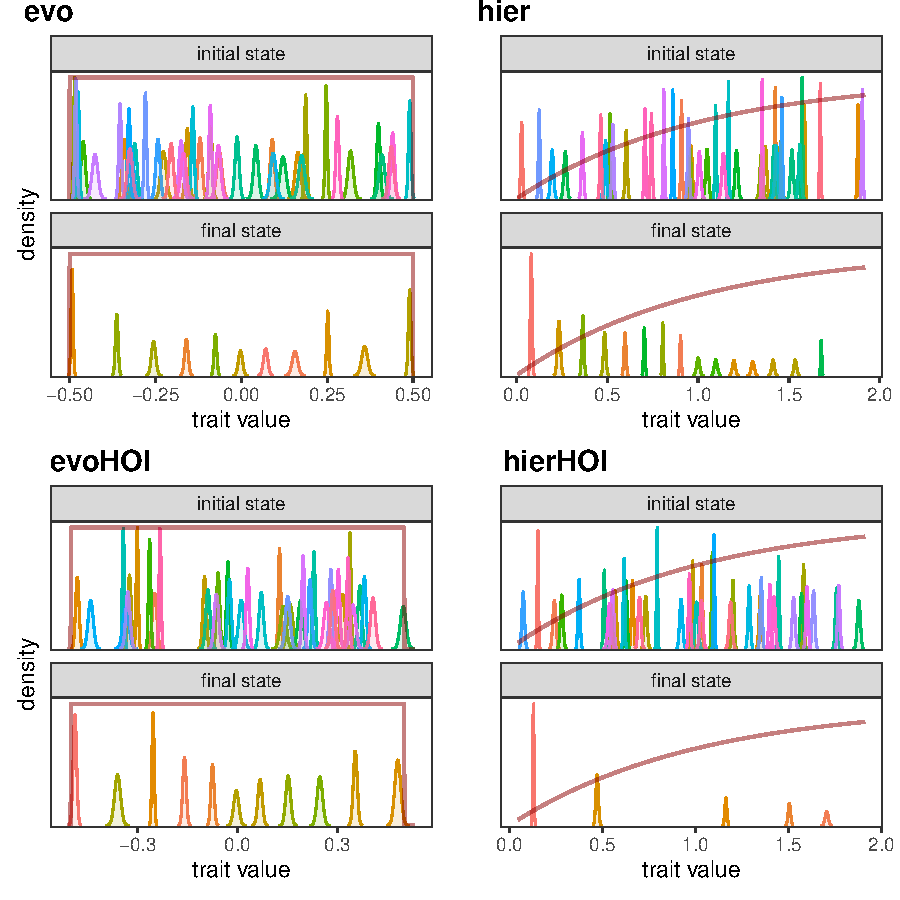
\includegraphics[width=\textwidth]{examples.pdf}
  \caption{Eco-evolutionary dynamics of many different species competing along a trait axis with four different types of species interactions: evo, evoHOI (evolutionary HOIs), hier (hierarchical pairwise model), hierHOI (hierarchical higher-order model). For each model, the top panel is the initial and the bottom panel the final, eco-evolutionary equilibrium distribution of species' traits along the one-dimensional trait axis. The red lines show the shape of the intrinsic growth rate function in each scenario (not drawn to scale). In each simulation, intraspecific trait standard deviations are low and $\omega = 0.1$; see Table~\ref{tab:params} for all other parameters.}
  \label{fig:examples}
\end{figure}


\begin{figure}[p]
  \centering
  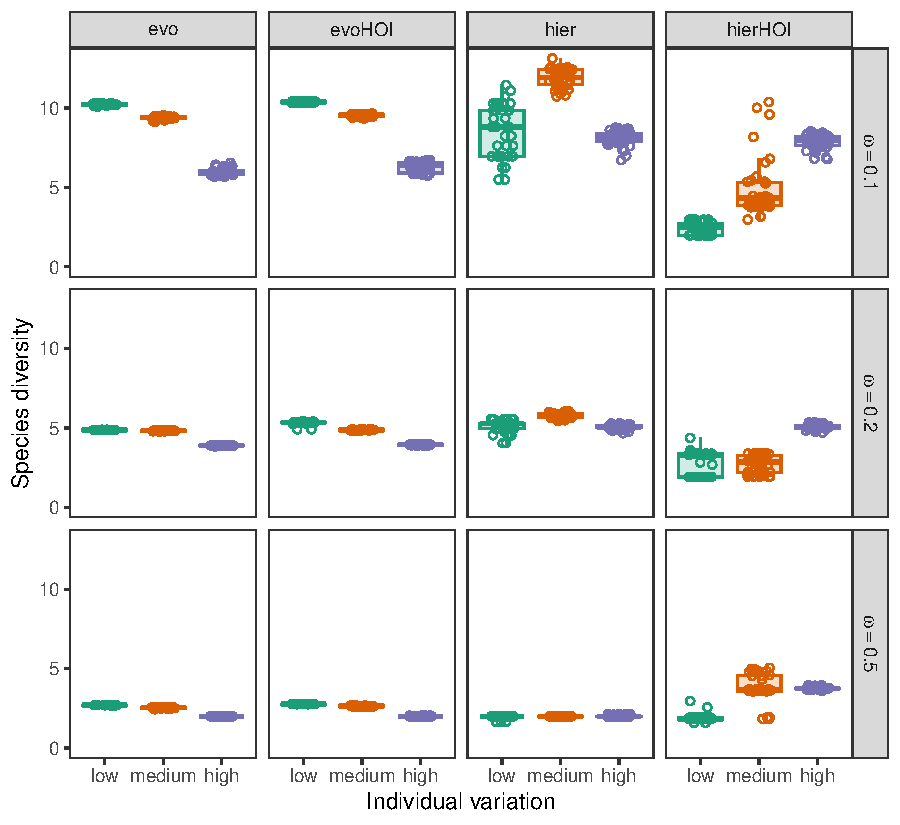
\includegraphics[width=\textwidth]{diversity.pdf}
  \caption{Effect of individual trait variation (x-axis), different competition widths (rows), and model choice (columns) on species richness. Box plots summarize the number of species that coexisted at the end of 40 replicate simulations; points show the actual individual simulation results (they have been jittered sideways to reduce overlap). Trait-based HOI models rarely lead to more species coexisting in comparison to pairwise models except when HOIs are hierarchical (hierHOI), the pairwise competition width is large ($\omega > 0.1$), and individual variation is not too low.}
  \label{fig:diversity}
\end{figure}


\begin{figure}[p]
  \centering
  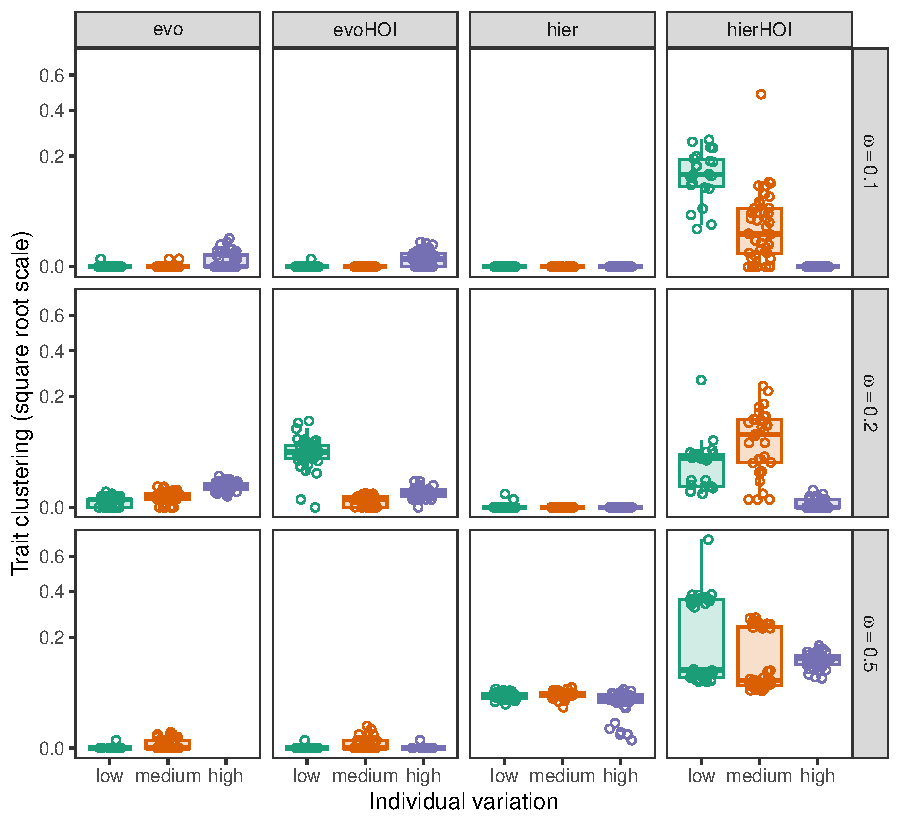
\includegraphics[width=\textwidth]{clustering.pdf}
  \caption{As Figure~\ref{fig:diversity}, but with trait clustering along the y-axis. A score close to 0 means the community's species are much more evenly spaced than expected by chance, while a score close to 1 means the opposite: the species are more clustered than expected. Pairwise models (evo, hier) and HOIs (evoHOI, hierHOI) all lead to very even trait spacing, although hierHOI can lead to somewhat higher clustering. The data are missing for the evo model at $\omega = 0.5$ and high individual variation because in that scenario, it was always two species surviving in all 40 replicates, so there is no meaningful measure of trait clustering in that case.}
  \label{fig:clustering}
\end{figure}


\begin{figure}[p]
  \centering
  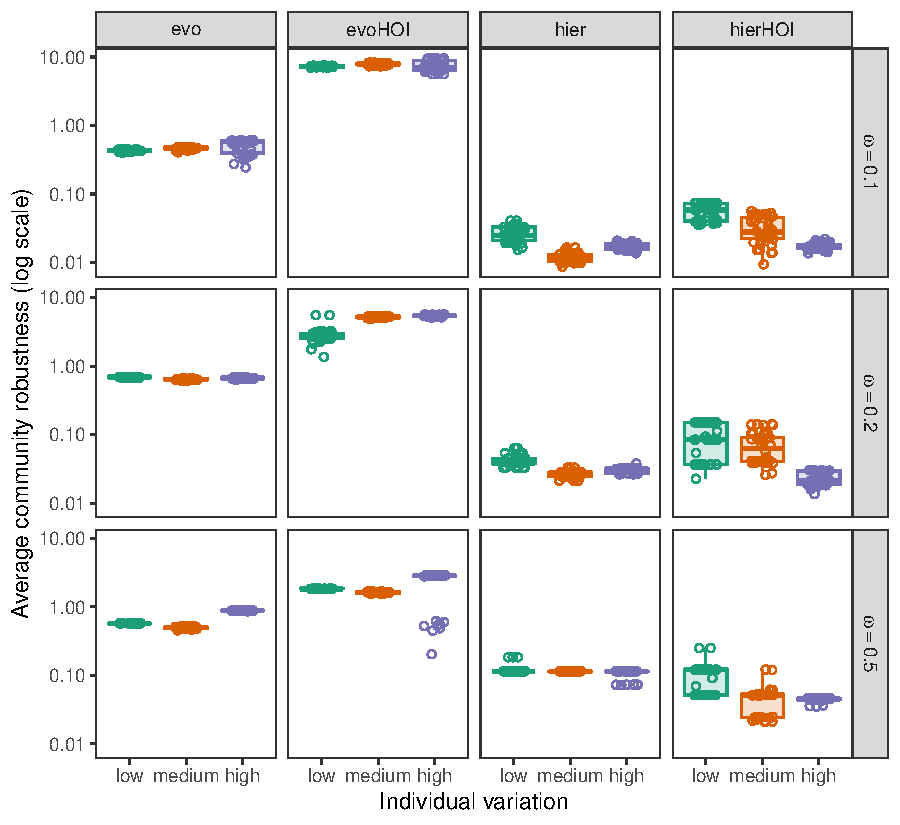
\includegraphics[width=\textwidth]{robustness.pdf}
  \caption{As Figure~\ref{fig:diversity}, but with average community robustness along the y-axis (on the log scale). Higher values denote higher community robustness against environmental perturbations.}
  \label{fig:robustness}
\end{figure}




\end{document}
